\documentclass{standalone}

\usepackage{TikzStyle}
\usepackage{mystyle}
\usetikzlibrary{automata}

\newcommand{\gpoint}[2]{%
\filldraw [gray] (#1,#2) circle [radius=2pt]
}

\begin{document}
    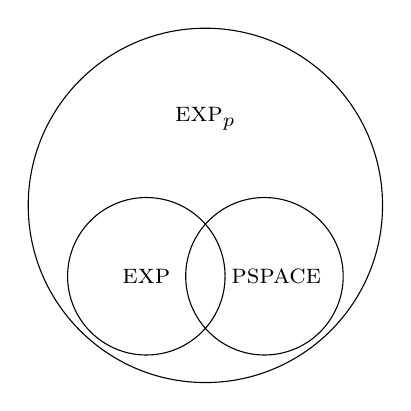
\begin{tikzpicture}
        %\node[draw,circle,inner sep=0.5cm] () at (0,0) {$\PClass$};
        \draw (-0.75,0) circle [radius=1cm];
        \draw (0.75,0) circle [radius=1cm];
        \draw (0,0.9) circle [radius=2.25cm];
        \node () at (-0.75,0) {$\textsc{exp}$};
        \node () at (0.9,0) {$\textsc{pspace}$};
        \node () at (0,2) {$\textsc{exp}_{p}$};
    \end{tikzpicture}
\end{document}
